\subsection*{1.1}
\subsubsection*{1.1.a}
The gradient can be calculated as follows:


% dsigma_j^2 / d_Xri
{\Large $\frac{\delta L^{(t)}}{\delta \textbf{W}_{ph}}$ }:
\boxed{\begin{aligned}
    \frac{\delta L^{(t)}}{\delta \textbf{W}_{ph}}
    &= \frac{\delta L^{(t)}}{\delta \hat{\textbf{y}}^{(t)}}
        \frac{\delta \hat{\textbf{y}}^{(t)}}{\delta \textbf{p}^{(t)}}
        \frac{\delta \textbf{p}^{(t)}}{\delta \textbf{W}_{ph}} \\
    &= \frac{\delta L^{(t)}}{\delta \hat{\textbf{y}}^{(t)}}
        \frac{\delta \hat{\textbf{y}}^{(t)}}{\delta \textbf{p}^{(t)}}
        \frac{\delta}{\delta \textbf{W}_{ph}} \textbf{W}_{ph} * h^{(t)} + b_{p} 
    &= \frac{\delta L^{(t)}}{\delta \hat{\textbf{y}}^{(t)}}
        \frac{\delta \hat{\textbf{y}}^{(t)}}{\delta \textbf{p}^{(t)}} h^{(t)}  \\
\end{aligned}}
\vspace{1cm}

\subsubsection*{1.1.b}
For the next gradient, we need to keep in mind the temporal and recursive nature. As such, we can define it as:
{\Large $\frac{\delta L^{(t)}}{\delta \textbf{W}_{hh}}$ }:
\boxed{\begin{aligned}
    \frac{\delta L^{(t)}}{\delta \textbf{W}_{hh}}
    &= \frac{\delta L^{(t)}}{\delta \hat{\textbf{y}}^{(t)}}
        \frac{\delta \hat{\textbf{y}}^{(t)}}{\delta \textbf{p}^{(t)}}
        \frac{\delta \textbf{p}^{(t)}}{\delta \textbf{h}^{(t)}} \\
        &= 
        \sum_{i=0}^{T=t}
        \frac{\delta L^{(t)}}{\delta \hat{\textbf{y}}^{(t)}}
        \frac{\delta \hat{\textbf{y}}^{(t)}}{\delta \textbf{p}^{(t)}}
        \frac{\delta \textbf{p}^{(t)}}{\delta \textbf{h}^{(t)}}
        \frac{\delta \textbf{h}^{(t)}}{\delta \textbf{h}_{i}}
        \frac{\delta \textbf{h}^{(i)}}{\delta \textbf{W}_{hh}} \\
    &=  \sum_{i=0}^{T=t}
        \frac{\delta L^{(t)}}{\delta \hat{\textbf{y}}^{(t)}}
        \frac{\delta \hat{\textbf{y}}^{(t)}}{\delta \textbf{p}^{(t)}}
        \frac{\delta \textbf{p}^{(t)}}{\delta \textbf{h}^{(t)}}
        \prod_{j=i+1}^{T} \Big( 
            \frac{\delta \textbf{h}^{(j)}}{\delta \textbf{h}_{j-1}}
        \Big)
        \frac{\delta \textbf{h}^{(i)}}{\delta \textbf{W}_{hh}} \\
\end{aligned}}
\vspace{1cm}

\subsection*{1.1.c}
There is a very clear distinction between the former formula and the latter: the derivative of the latter
does not depend on the previous time-steps. Essentially, the matrix mapping the output only depends on the last
hidden state. When you compare this to the recursive nature of $\frac{\delta L^{(t)}}{\delta \textbf{W}_{hh}}$, 
one important practical difference becomes clear: how "far" the gradient has to traverse to update the weights. For
$W_{ph}$, the gradient depends only on the latest hidden state, which means that the gradient and updates
generally are stronger. With $W_{hh}$, however, the jacobian product intuitievly either "explodes" the
gradient, or it weakens it, "vanishing" the gradient in the process the more time-steps we go back, due to 
its recursive nature.

\subsection*{1.2}
\subsubsection*{1.2.a}
Gates, go as follow:

\begin{enumerate}
    \item Input modulation gate: this gate is responsible for actually calculating new values that 
    are going to be eventually added to the cell-state. These values are modulated further with tanh,
    as to ensure that gradients remain stable by not exceeding 1 / -1 (as tanh does).
    \item Input gate: this gate acts as "differentiable" mask for the input modulation gate.
    It decides how much of the input modulation gate will be added on top of the current cell state.
    The sigmoid allows this "mask-like" functionality to be applied, ranging between 0 and 1.
    \item Forget gate: this gate is responsible for deciding how much of the previous cell state
    still remains (based on the current input and hidden state). It does so, again, by using
    sigmoids' range of 0 and 1 to decide whether to maintain nothing (0) or all (1).
    \item Output gate: this gate uses another "sigmoid-mask" to decide how much of the cell-state
    is used as hidden-state, possibly more short-term oriented. Before that, the cell-state
    is put through tanh to ensure that the value after its previous update is more stable again, max 1.
\end{enumerate}

\subsubsection*{1.2.b}
The number of parameters are $4 * \Big((N_{hidden} * N_{hidden}) + (N_{hidden} * N_{input}) 
+ N_{hidden}\Big) + (N_{hidden} * N_{output}) $.

\subsubsection*{1.3}
During training, the model was trained a number of times. To be more specific, the model was trained on three seeds (42, 1337 and 1994), with varying
sequence lengths eventually becoming 41 and 81 ((10, 20) * 4 + 2 -1). Both the training loss and training accuracy can be seen in the figure below, where
the standard deviation for every 10th step defines the "error-boundary", across seeds. Two noticeable differences occur. Whereas
sequences of 41 lenght eventually reach a proper convergence (across all seeds), sequences twice as long
still have a very high variance in both loss and and accuracy. However, this might be a simple shift of increased
variance that sequences of length 41 had (from timestep 500(=50*10) to 2000(=200*10)); if the model were to continue
to train, the model might reach similar convergence.

\begin{figure}[h]%
    \centering
    \subfloat[\centering LSTM accuracy averaged]{{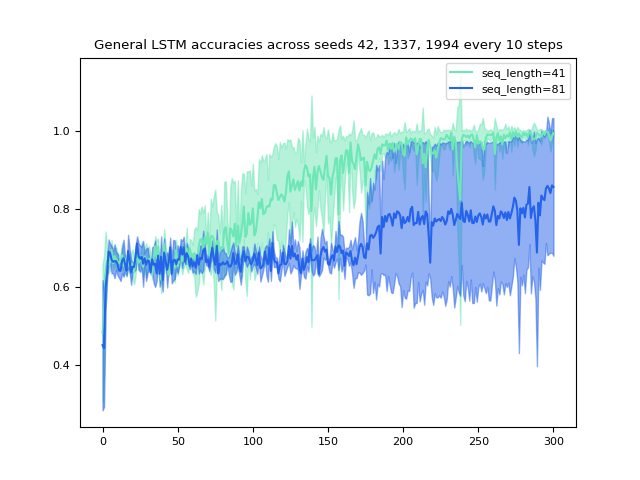
\includegraphics[width=6.5cm]{images/LSTM-plot-accs.png} }}%
    \qquad
    \subfloat[\centering LSTM loss averaged]{{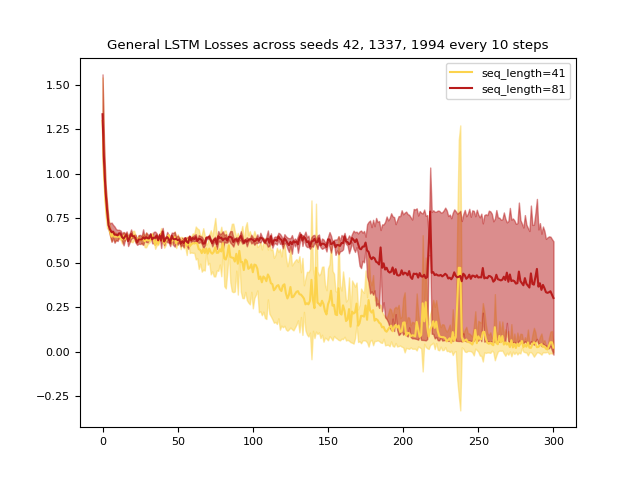
\includegraphics[width=6.5cm]{images/LSTM-plot-loss.png} }}%
    \caption{LSTM Performance over time: note, these are estimates stored every 10 steps of (3000), thus showing 300 recordings}%
    \label{fig:defaults}%
\end{figure}

\subsubsection*{1.4}
Now, with PeepLSTM, the results across sequence lengths look more similar to one another. The mean performance for 
both the longer sequence and shorter sequence seem to be much closer now, hinting at the idea that the peepholes
may make models more robust in general for longer sequences (even if the variance is still relatively high). What's
more, the signal averages seem more noisy, indicating slightly less stable predictions in general (notice both
losses and accuracies seem to be contain more discord). The true power of the peephole LSTM is mostly visible
when looking at the general increase in performance speed for lenght 81: where the vanilla seemed to plateau for
a while (likely due to the output gate being closed), Peephole LSTMS bypass some of the problems by provind this extra signal.

\begin{figure}[h]%
    \centering
    \subfloat[\centering PeepLSTM accuracy averaged]{{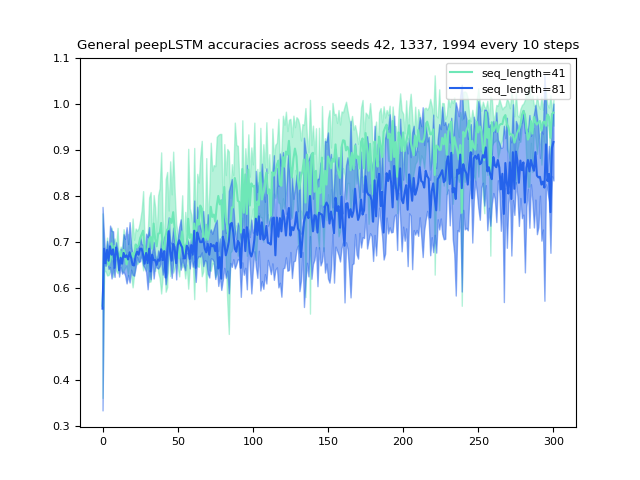
\includegraphics[width=6.5cm]{images/peepLSTM-plot-accs.png} }}%
    \qquad
    \subfloat[\centering PeepLSTM loss averaged]{{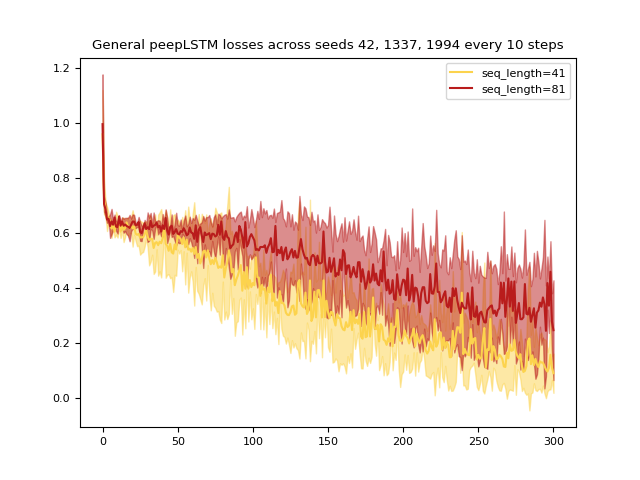
\includegraphics[width=6.5cm]{images/peepLSTM-plot-loss.png} }}%
    \caption{PeepLSTM Performance over time: note, these are estimates stored every 10 steps of (3000), thus showing 300 recordings}%
    \label{fig:defaults}%
\end{figure}
